%%
%% This is file `sample-sigplan.tex',
%% generated with the docstrip utility.
%%
%% The original source files were:
%%
%% samples.dtx  (with options: `sigplan')
%% 
%% IMPORTANT NOTICE:
%% 
%% For the copyright see the source file.
%% 
%% Any modified versions of this file must be renamed
%% with new filenames distinct from sample-sigplan.tex.
%% 
%% For distribution of the original source see the terms
%% for copying and modification in the file samples.dtx.
%% 
%% This generated file may be distributed as long as the
%% original source files, as listed above, are part of the
%% same distribution. (The sources need not necessarily be
%% in the same archive or directory.)
%%
%%
%% Commands for TeXCount
%TC:macro \cite [option:text,text]
%TC:macro \citep [option:text,text]
%TC:macro \citet [option:text,text]
%TC:envir table 0 1
%TC:envir table* 0 1
%TC:envir tabular [ignore] word
%TC:envir displaymath 0 word
%TC:envir math 0 word
%TC:envir comment 0 0
%%
%%
%% The first command in your LaTeX source must be the \documentclass
%% command.
%%
%% For submission and review of your manuscript please change the
%% command to \documentclass[manuscript, screen, review]{acmart}.
%%
%% When submitting camera ready or to TAPS, please change the command
%% to \documentclass[sigconf]{acmart} or whichever template is required
%% for your publication.
%%
%%
\documentclass[sigplan,acmsmall,manuscript,anonymous,screen,review]{acmart}

%%
%% \BibTeX command to typeset BibTeX logo in the docs
\AtBeginDocument{%
  \providecommand\BibTeX{{%
    Bib\TeX}}}

%% Rights management information.  This information is sent to you
%% when you complete the rights form.  These commands have SAMPLE
%% values in them; it is your responsibility as an author to replace
%% the commands and values with those provided to you when you
%% complete the rights form.
\setcopyright{acmcopyright}
\copyrightyear{2018}
\acmYear{2018}
\acmDOI{XXXXXXX.XXXXXXX}

%% These commands are for a PROCEEDINGS abstract or paper.
\acmConference[Conference acronym 'XX]{Make sure to enter the correct
  conference title from your rights confirmation emai}{June 03--05,
  2018}{Woodstock, NY}
%%
%%  Uncomment \acmBooktitle if the title of the proceedings is different
%%  from ``Proceedings of ...''!
%%
%%\acmBooktitle{Woodstock '18: ACM Symposium on Neural Gaze Detection,
%%  June 03--05, 2018, Woodstock, NY}
\acmPrice{15.00}
\acmISBN{978-1-4503-XXXX-X/18/06}


%%
%% Submission ID.
%% Use this when submitting an article to a sponsored event. You'll
%% receive a unique submission ID from the organizers
%% of the event, and this ID should be used as the parameter to this command.
%%\acmSubmissionID{123-A56-BU3}

%%
%% For managing citations, it is recommended to use bibliography
%% files in BibTeX format.
%%
%% You can then either use BibTeX with the ACM-Reference-Format style,
%% or BibLaTeX with the acmnumeric or acmauthoryear sytles, that include
%% support for advanced citation of software artefact from the
%% biblatex-software package, also separately available on CTAN.
%%
%% Look at the sample-*-biblatex.tex files for templates showcasing
%% the biblatex styles.
%%

%%
%% The majority of ACM publications use numbered citations and
%% references.  The command \citestyle{authoryear} switches to the
%% "author year" style.
%%
%% If you are preparing content for an event
%% sponsored by ACM SIGGRAPH, you must use the "author year" style of
%% citations and references.
%% Uncommenting
%% the next command will enable that style.
%%\citestyle{acmauthoryear}


%%
%% end of the preamble, start of the body of the document source.
\begin{document}

%%
%% The "title" command has an optional parameter,
%% allowing the author to define a "short title" to be used in page headers.
\title{The Name of the Title Is Hope}

%%
%% The "author" command and its associated commands are used to define
%% the authors and their affiliations.
%% Of note is the shared affiliation of the first two authors, and the
%% "authornote" and "authornotemark" commands
%% used to denote shared contribution to the research.
\author{Ben Trovato}
\authornote{Both authors contributed equally to this research.}
\email{trovato@corporation.com}
\orcid{1234-5678-9012}
\author{G.K.M. Tobin}
\authornotemark[1]
\email{webmaster@marysville-ohio.com}
\affiliation{%
  \institution{Institute for Clarity in Documentation}
  \streetaddress{P.O. Box 1212}
  \city{Dublin}
  \state{Ohio}
  \country{USA}
  \postcode{43017-6221}
}

\author{Lars Th{\o}rv{\"a}ld}
\affiliation{%
\institution{The Th{\o}rv{\"a}ld Group}
\streetaddress{1 Th{\o}rv{\"a}ld Circle}
\city{Hekla}
\country{Iceland}}
\email{larst@affiliation.org}

\author{Valerie B\'eranger}
\affiliation{%
  \institution{Inria Paris-Rocquencourt}
  \city{Rocquencourt}
  \country{France}
}

\author{Aparna Patel}
\affiliation{%
  \institution{Rajiv Gandhi University}
  \streetaddress{Rono-Hills}
  \city{Doimukh}
  \state{Arunachal Pradesh}
  \country{India}}

\author{Huifen Chan}
\affiliation{%
  \institution{Tsinghua University}
  \streetaddress{30 Shuangqing Rd}
  \city{Haidian Qu}
  \state{Beijing Shi}
  \country{China}}

\author{Charles Palmer}
\affiliation{%
  \institution{Palmer Research Laboratories}
  \streetaddress{8600 Datapoint Drive}
  \city{San Antonio}
  \state{Texas}
  \country{USA}
  \postcode{78229}}
\email{cpalmer@prl.com}

\author{John Smith}
\affiliation{%
\institution{The Th{\o}rv{\"a}ld Group}
\streetaddress{1 Th{\o}rv{\"a}ld Circle}
\city{Hekla}
\country{Iceland}}
\email{jsmith@affiliation.org}

\author{Julius P. Kumquat}
\affiliation{%
  \institution{The Kumquat Consortium}
  \city{New York}
  \country{USA}}
\email{jpkumquat@consortium.net}

%%
%% By default, the full list of authors will be used in the page
%% headers. Often, this list is too long, and will overlap
%% other information printed in the page headers. This command allows
%% the author to define a more concise list
%% of authors' names for this purpose.
\renewcommand{\shortauthors}{Trovato et al.}

%%
%% The abstract is a short summary of the work to be presented in the
%% article.
\begin{abstract}
  A clear and well-documented \LaTeX\ document is presented as an
  article formatted for publication by ACM in a conference proceedings
  or journal publication. Based on the ``acmart'' document class, this
  article presents and explains many of the common variations, as well
  as many of the formatting elements an author may use in the
  preparation of the documentation of their work.
\end{abstract}

%%
%% The code below is generated by the tool at http://dl.acm.org/ccs.cfm.
%% Please copy and paste the code instead of the example below.
%%
\begin{CCSXML}
  <ccs2012>
  <concept>
  <concept_id>10010520.10010553.10010562</concept_id>
  <concept_desc>Computer systems organization~Embedded systems</concept_desc>
  <concept_significance>500</concept_significance>
  </concept>
  <concept>
  <concept_id>10010520.10010575.10010755</concept_id>
  <concept_desc>Computer systems organization~Redundancy</concept_desc>
  <concept_significance>300</concept_significance>
  </concept>
  <concept>
  <concept_id>10010520.10010553.10010554</concept_id>
  <concept_desc>Computer systems organization~Robotics</concept_desc>
  <concept_significance>100</concept_significance>
  </concept>
  <concept>
  <concept_id>10003033.10003083.10003095</concept_id>
  <concept_desc>Networks~Network reliability</concept_desc>
  <concept_significance>100</concept_significance>
  </concept>
  </ccs2012>
\end{CCSXML}

\ccsdesc[500]{Computer systems organization~Embedded systems}
\ccsdesc[300]{Computer systems organization~Redundancy}
\ccsdesc{Computer systems organization~Robotics}
\ccsdesc[100]{Networks~Network reliability}

%%
%% Keywords. The author(s) should pick words that accurately describe
%% the work being presented. Separate the keywords with commas.
\keywords{datasets, neural networks, gaze detection, text tagging}
%% A "teaser" image appears between the author and affiliation
%% information and the body of the document, and typically spans the
%% page.
\begin{teaserfigure}
  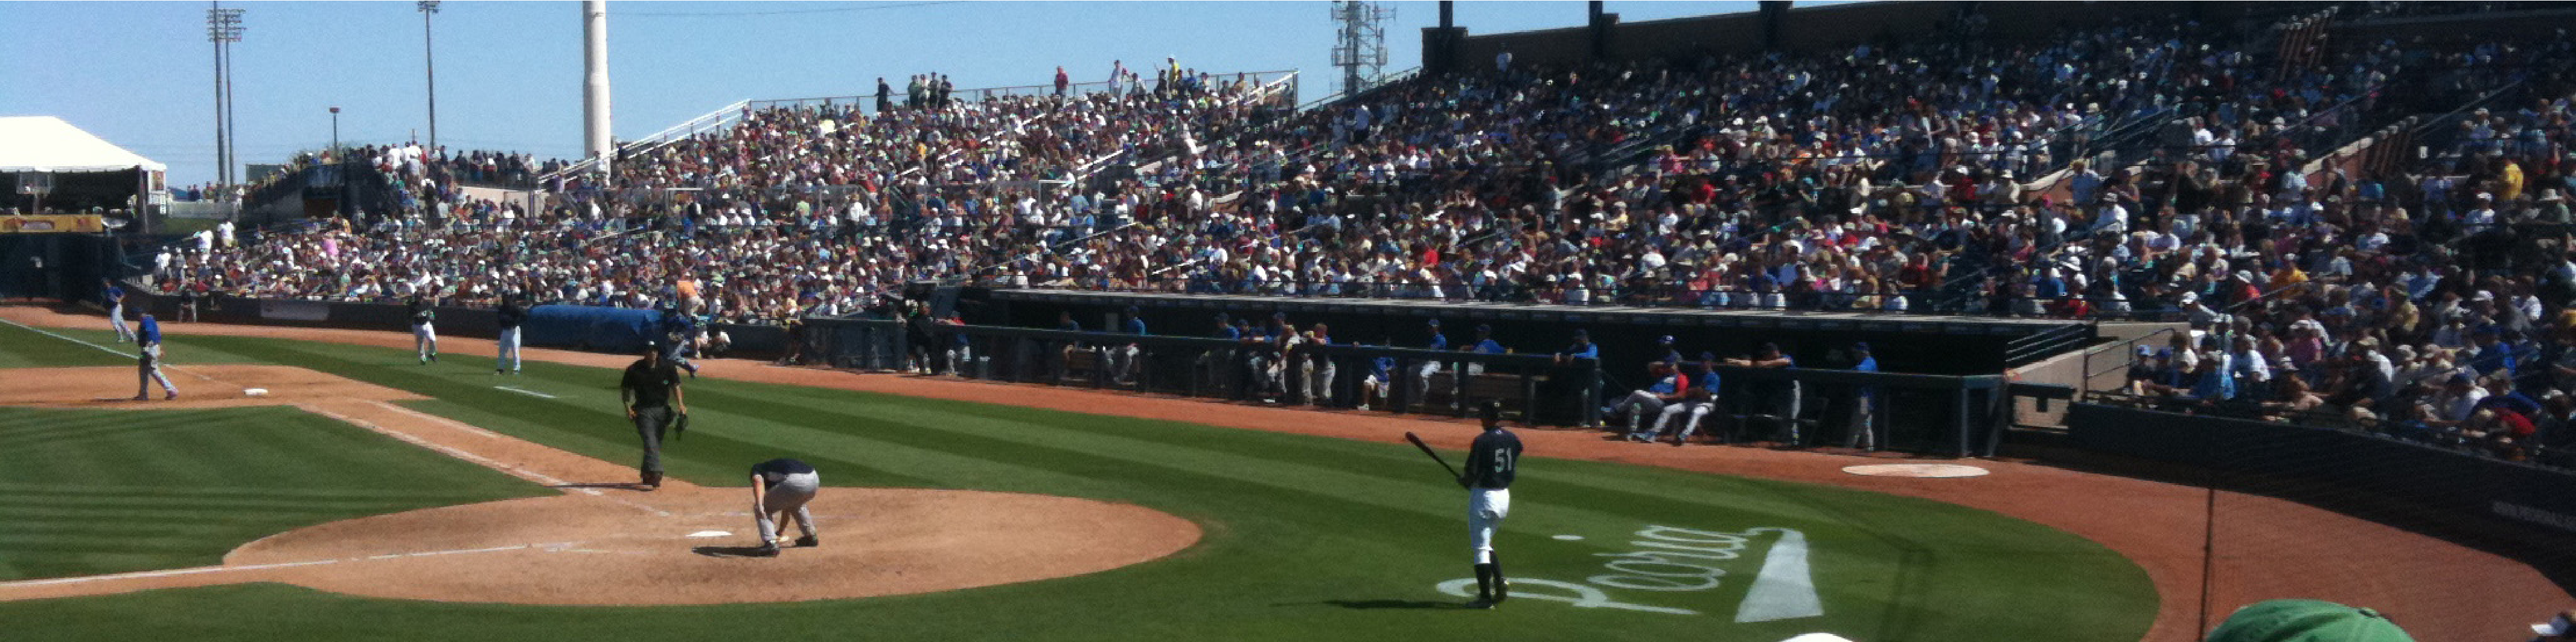
\includegraphics[width=\textwidth]{sampleteaser}
  \caption{Seattle Mariners at Spring Training, 2010.}
  \Description{Enjoying the baseball game from the third-base
    seats. Ichiro Suzuki preparing to bat.}
  \label{fig:teaser}
\end{teaserfigure}

\received{20 February 2007}
\received[revised]{12 March 2009}
\received[accepted]{5 June 2009}

%%
%% This command processes the author and affiliation and title
%% information and builds the first part of the formatted document.
\maketitle

\section{Introduction}

Language-oriented programming (LOP)\cite{LOP} is solving a class of problems by designing one or more new domain-specific languages (DSLs).
To avoid building common languages constructs like loops and branches,
developers may implement DSLs on top of another general-purpose programming language (called host language).
Developers can extend the host language based on the language features, rendering programs with domain-specific forms.
Languages with features like macros and higher-order functions are frequently employed.
By specifying translation rules from the DSL to the host language, developers can obtain a DSL interpreter naturally.
This type of DSL is called embedded DSL (eDSL).

Despite eDSL can significantly reduce implementation costs, DSL users find it inconvenient due to the inevitable need to learn the host language and understand error messages.
This is called abstraction leakage, where the users writes a program in DSL and it is translated into the host language,
causing the program executed formally differently from the original program.
Much prior work has focused on how to translate information from the host language to the DSL users manually.
\todo{More related work about generate information manually}

Pombrio et al. \cite{resugar} have made a great progress in maintenance of abstraction automatically.
They proposed \textit{resugaring}, by selectively reorganizing the sequence of evaluations on the host language to the DSL according to the reverse translation rules.
But there are several practical problems in this approach.
First, programs with a lot of syntactic sugars are pretty expensive to check whether each term in the evaluation sequences can be resugared.
Second, it still contains a host language evaluator executing,
so that users cannot intuit the functionality of language constructs.
Yang et al. \cite{lazy-desg} have solved the first problem via lazy desugaring.

% In this paper, we will focus on the second problem.
% In this paper, we propose a new approach to implementing DSLs by translation rules but make it standalone.

In general, embedded DSLs treat the host language as a black box.
We take the semantics of the host language as a white box, written by the meta language,
and derive the semantics for language constructs of DSL automatically.

We follow the core ideas of inferring type rules for syntactic sugars \cite{infer-types} and extend it to the semantics.
For example, in a host language with lambda abstraction and application, we can define $\<let>$ by translation rule:
\[ e_1~\<and>~e_2 => \<if>~e_1~\<then>~e_2~\<else>~\<false>. \]
The derivation of $\<and>$ is given in Fig. \ref{fig:and}.
In DSL, an expression matching the pattern of left-hand side (LHS) evaluates to $v$, if and only if the right-hand side (RHS) evaluates to $v$ (Step 1).
Based on the rules of if-then-else, we can futher expand the evaluation of RHS.
Since if-then-else is described in two rules according to the evaluation of $e_1$,
our derivation tree have to do the same thing (Step 2).
Similarly, the rule of $\<false>$ can be applied (Step 3).
Hence, we can obtain the following conclutions:
\[
  \inference{e_1 \Da \<true> & e_2 \Da v}
  {e_1~\<and>~e_2 \Da v}
  \qquad
  \inference{e_1 \Da \<false>}
  {e_1~\<and>~e_2 \Da \<false>}
\]
It should be observed that without mentioning $\<if>$, the rules directly describe the rules of $\<and>$.
That means, the abstraction we want to maintain --- that the rules of $\<and>$ are independent of the host language --- is true.

\begin{figure}[t!]
  \[
    \inference[(Step 1) ]{%
      \inference[(Step 2) ]{%
        e_1 \Da \<true>
        & e_2 \Da v
      }
      {\<if>~e_1~\<then>~e_2~\<else>~\<false> \Da v}
    }
    {e_1~\<and>~e_2 \Da v}
    \qquad
    \inference[(Step 1) ]{%
      \inference[(Step 2) ]{%
        e_1 \Da \<false>
        & \inference[(Step 3)]{}{\<false> \Da \<false>}
      }
      {\<if>~e_1~\<then>~e_2~\<else>~\<false> \Da \<false>}
    }
    {e_1~\<and>~e_2 \Da \<false>}
  \]
  \caption{Derivation of $\mathbf{and}$}
  \label{fig:and}
\end{figure}

It is seemingly natural but we are facing three challenges:
(1) Unlike type rules, which can typically be stated by one single rule,
many evaluation rules, such as $\<if>$, do not conform this property.
This may lead to nondeterminacy when searching rules or exponential growth in the number of rules.
(2) Most type rules are defined in a modular way,
which means the type of an expression depends on the types of subexpressions,
but the semantics may be not.
In particular, when using lambda-calculus as the host language,
lambda abstraction itself is a value.
Translation rules defined by lambda abstraction, is a value itself.
The evaluation rules of them may ruin the abstraction, like
\[ \<andf> => λx:\<bool>,y:\<bool>.~\<if>~x~\<then>~y~\<else>~\<false>. \]
(3) Since the rules of application include substitution,
we must specify the behavior of the expression containing substitution in semantic derivation.

To address challenge (1),
we introduce a variant of Skeleton \cite{skeleton} as meta-language to describe semantics.
Make sure that each language structure is evaluated according to unique rules,
in order to guarantee the determinacy of semantic derivation.
To address challenge (2),
we propose lambda lifting, to reveal the semantics of lambda abstraction.
To address challenge (3),
we show that substitution can maintain the correctness and abstraction of semantic derivation,
but we shall impose greater limitations on translation rules.

In this paper, we propose a new framework for DSL design.
We use simply-typed lambda-calculus (STLC) as the host language for its elementariness and versatility.
To increase the generality of the framework,
we provide meta-extensions (to introduce new vocabularies) and monad-extensions (to introduce side-effects) on the host language.
Then, users can specify DSL constructs by translation rules on the new extended host language.
Hence, as the focus of this paper, the framework will derive the evaluation rules and type rules for these constructs automatically, to make the DSL standalone.
All the semantics are described by the meta-language, and those of DSLs are generated.
Finally and naturally, our framework will generate interpreters based on semantics.
Our main technical contributions can be summarized as follows:

\begin{itemize}
  \item \todo{host}
  \item \todo{dsl}
  \item We present an algorithm to derive semantics for DSL constructs defined by translation rules.
        For the translation rules defined with lambda abstraction,
        we will give the lambda-lifting method.
        We will prove the correctness and abstraction of the algorithm.
  \item We give an implementation of the framework.
\end{itemize}


\end{document}
\endinput
%%
%% End of file `sample-sigplan.tex'.
